\chapter{Experimental Results}

%\begin{figure}
%  \centering
%    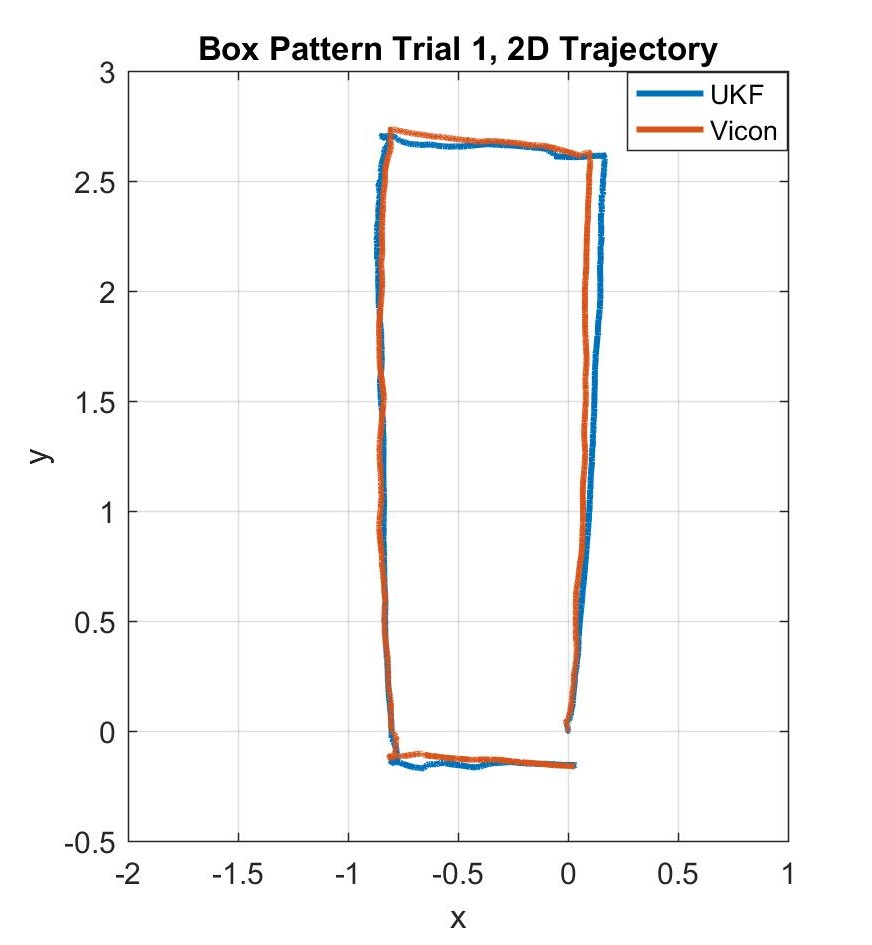
\includegraphics[width=0.5\textwidth]{box1_2d}
%  \caption[Box Pattern Trial 1, 2D Trajectory]{The two-dimensional projection of the first box pattern trajectory.}
%  \label{fig:box1_2d}
%\end{figure}

\begin{figure}
    \centering
    \begin{subfigure}{0.4\textwidth}
        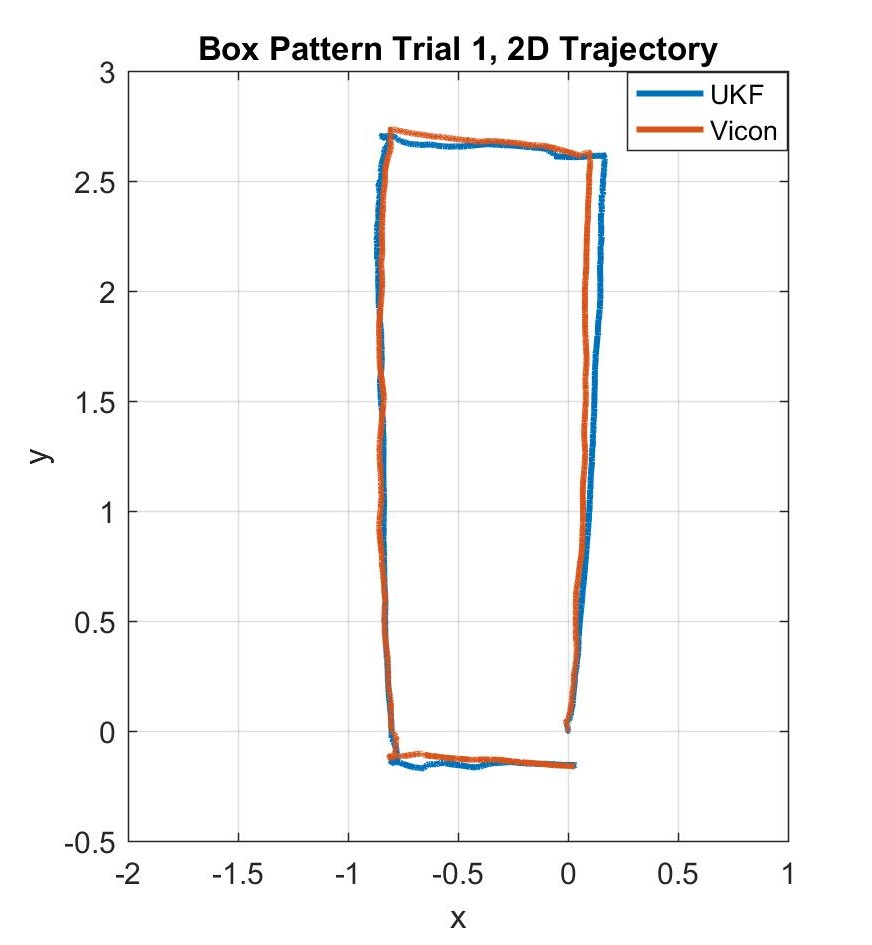
\includegraphics[width=\textwidth,left]{box1_2d}
    \end{subfigure}%
    ~ 
    \begin{subfigure}{0.6\textwidth}
        \centering
        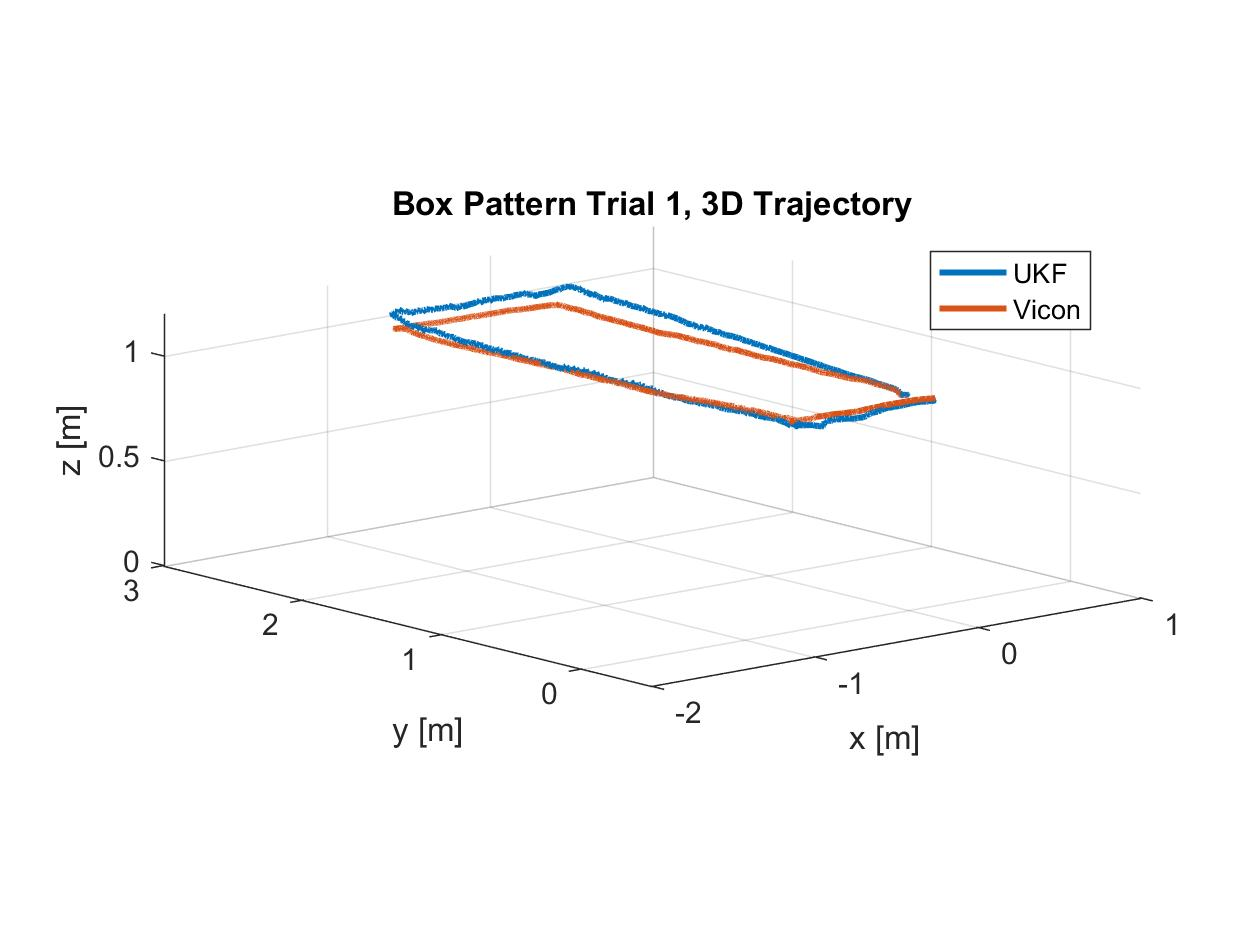
\includegraphics[width=\textwidth,right]{box1_3d}
    \end{subfigure}
    \caption[Box Pattern Trial 1 Trajectory]{2D and 3D trajectory plots from Box Pattern Trial~1.}
    \label{box1_traj}
\end{figure}

\begin{figure}
    \centering
    \begin{subfigure}{0.4\textwidth}
        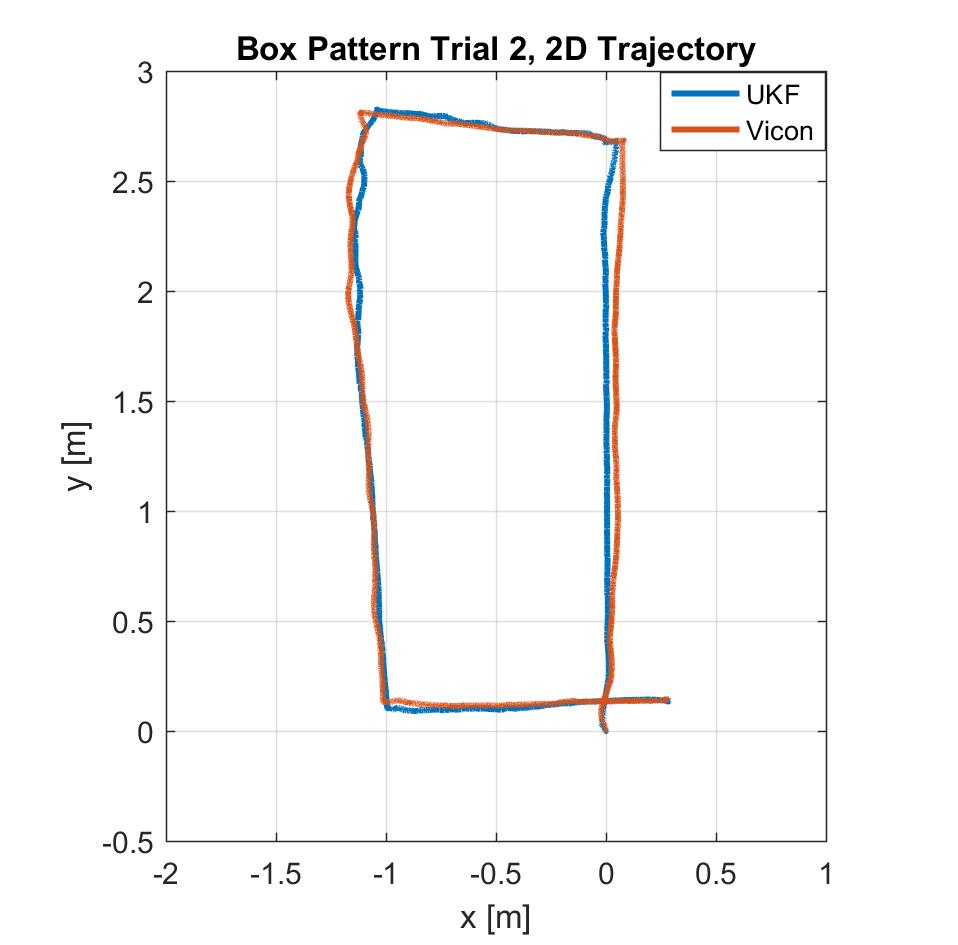
\includegraphics[width=\textwidth,left]{box2_2d}
    \end{subfigure}%
    ~ 
    \begin{subfigure}{0.6\textwidth}
        \centering
        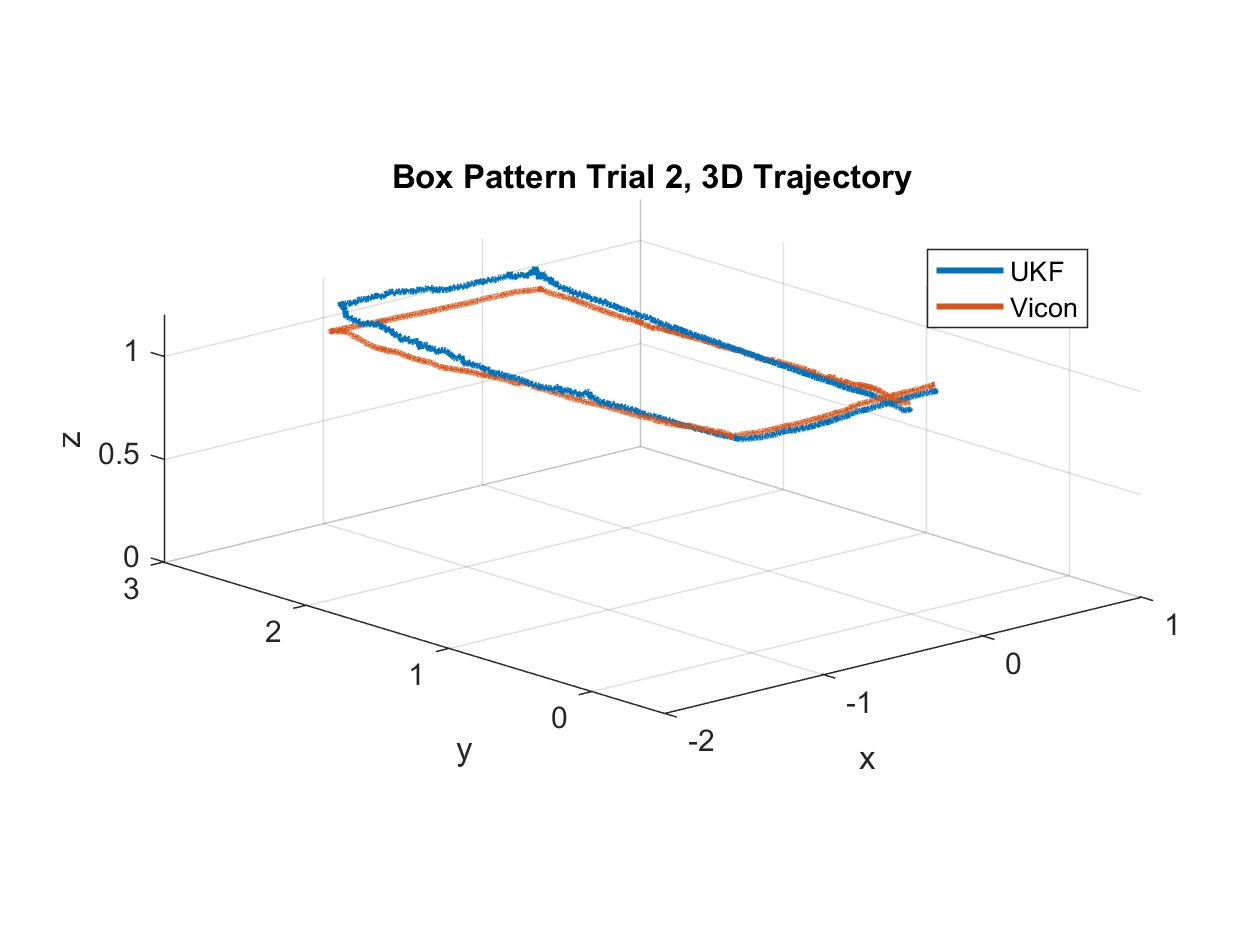
\includegraphics[width=\textwidth,right]{box2_3d}
    \end{subfigure}
    \caption[Box Pattern Trial 2 Trajectory]{2D and 3D trajectory plots from Box Pattern Trial~2.}
    \label{box2_traj}
\end{figure}

\begin{figure}
    \centering
    \begin{subfigure}{0.4\textwidth}
        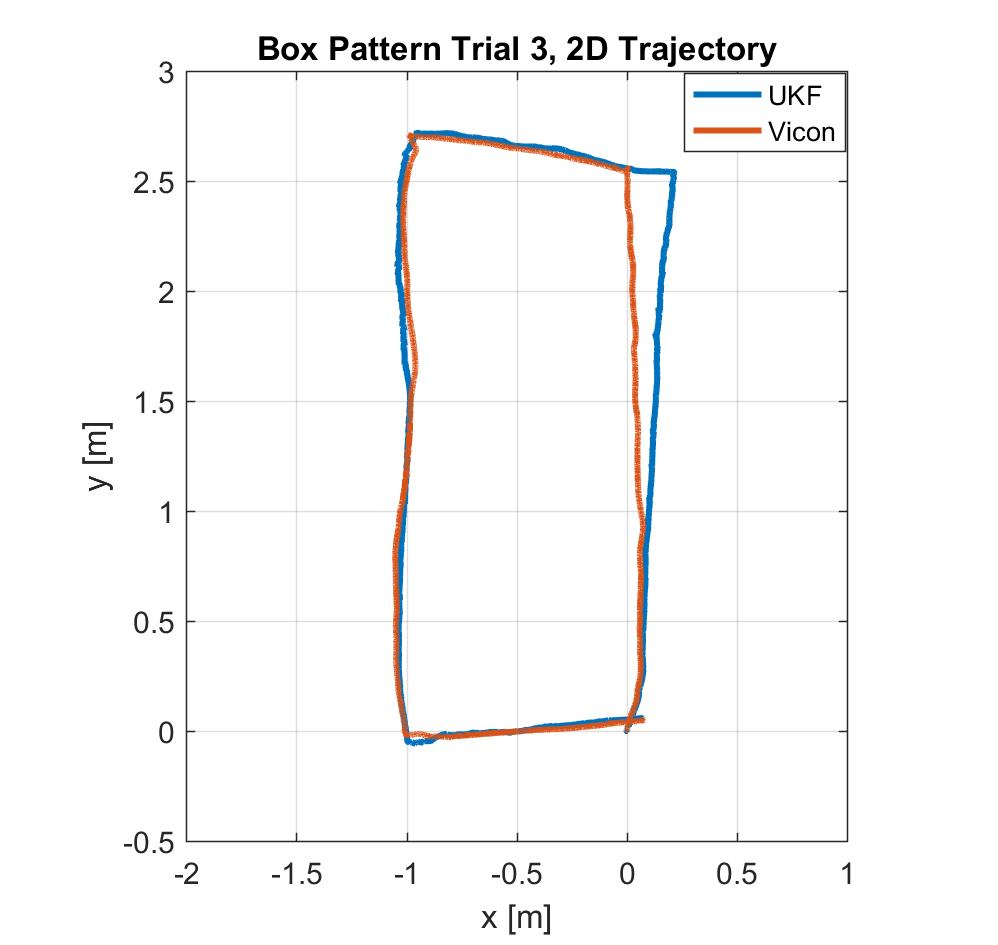
\includegraphics[width=\textwidth,left]{box3_2d}
    \end{subfigure}%
    ~ 
    \begin{subfigure}{0.6\textwidth}
        \centering
        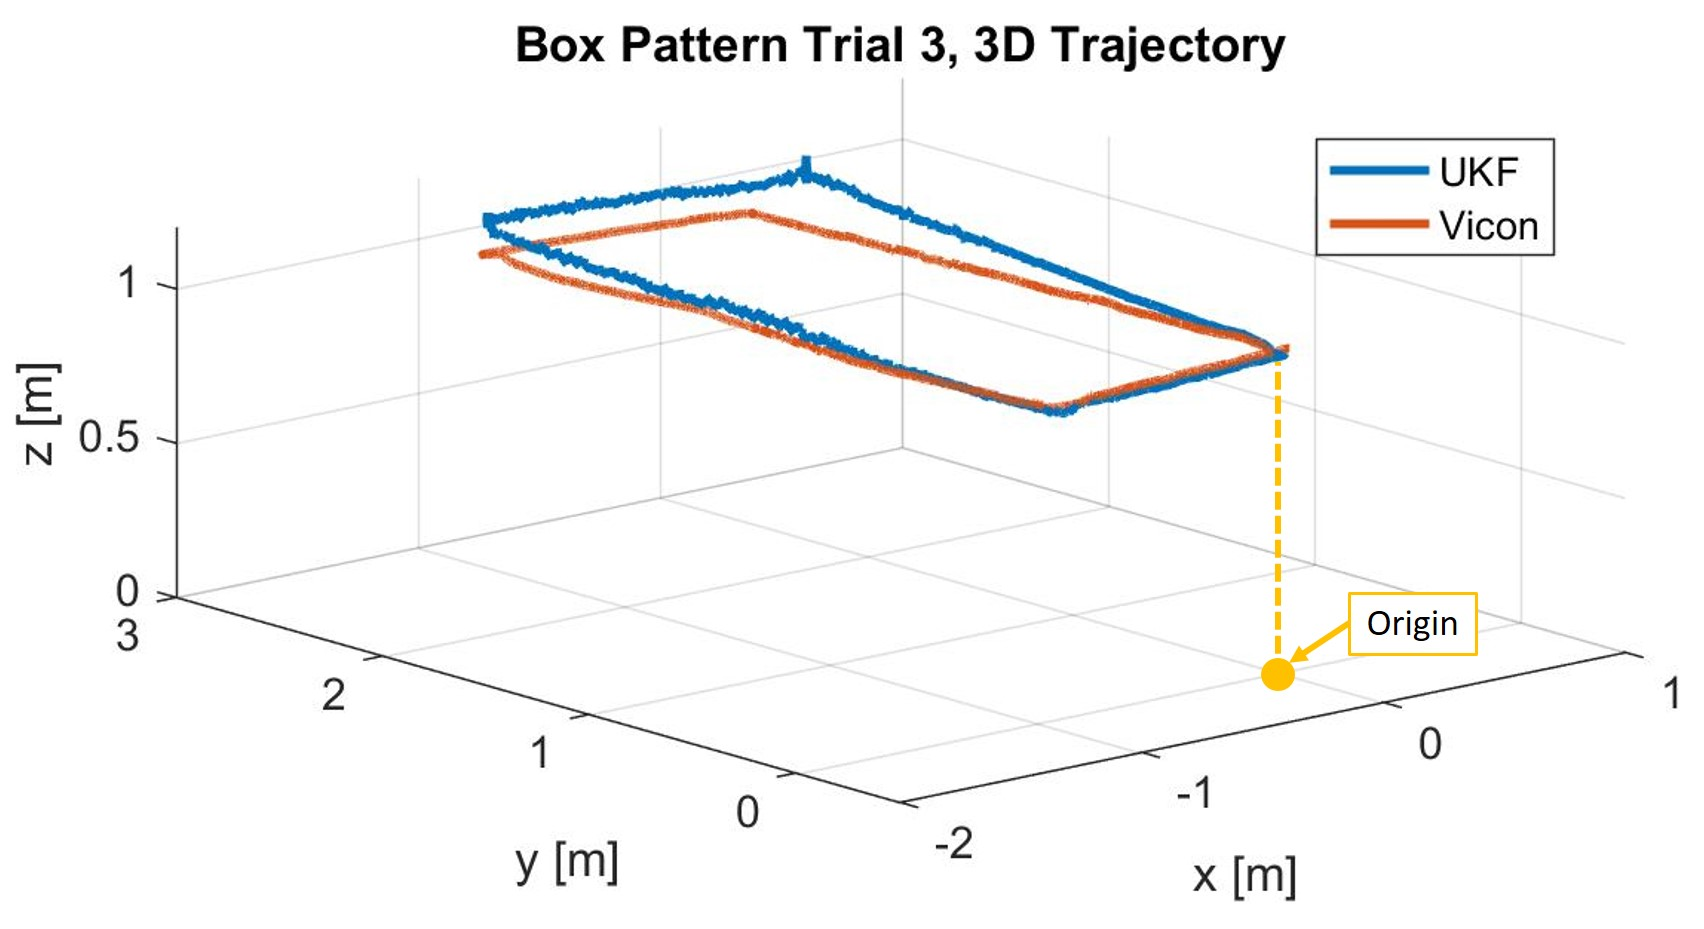
\includegraphics[width=\textwidth,right]{box3_3d}
    \end{subfigure}
    \caption[Box Pattern Trial 3 Trajectory]{2D and 3D trajectory plots from Box Pattern Trial~3.}
    \label{box3_traj}
\end{figure}

\begin{figure}
    \centering
    \begin{subfigure}{0.4\textwidth}
        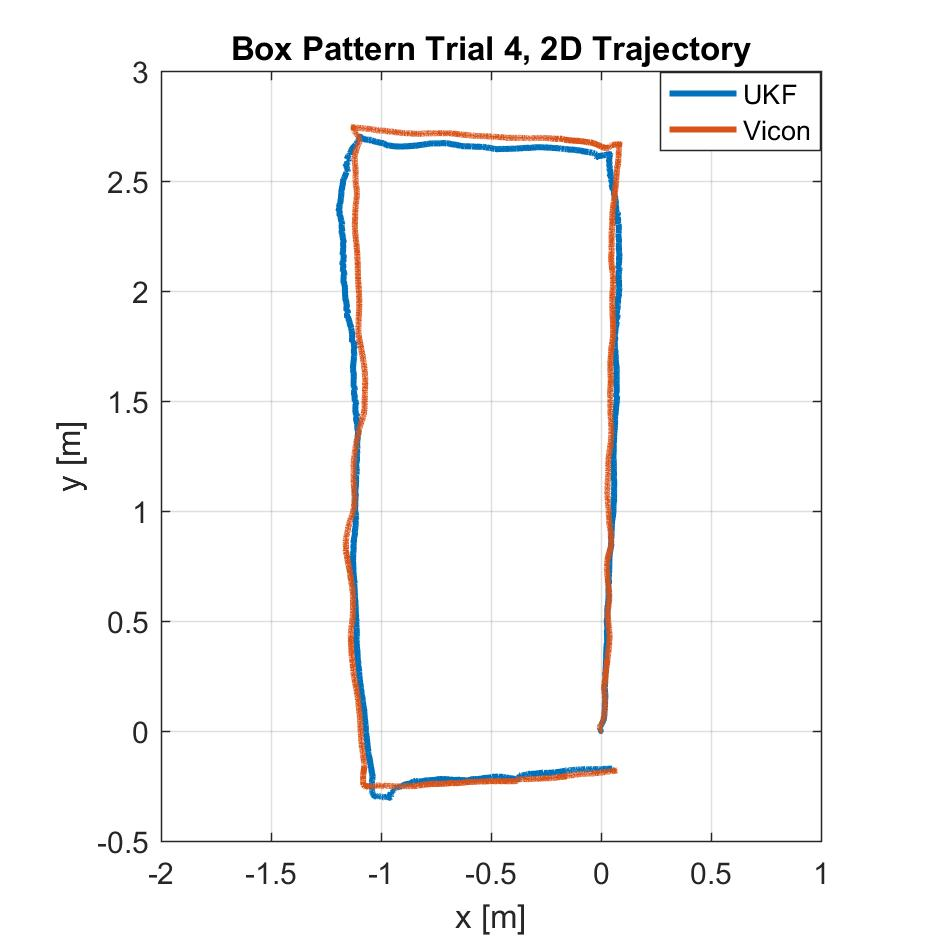
\includegraphics[width=\textwidth,left]{box4_2d}
    \end{subfigure}%
    ~ 
    \begin{subfigure}{0.6\textwidth}
        \centering
        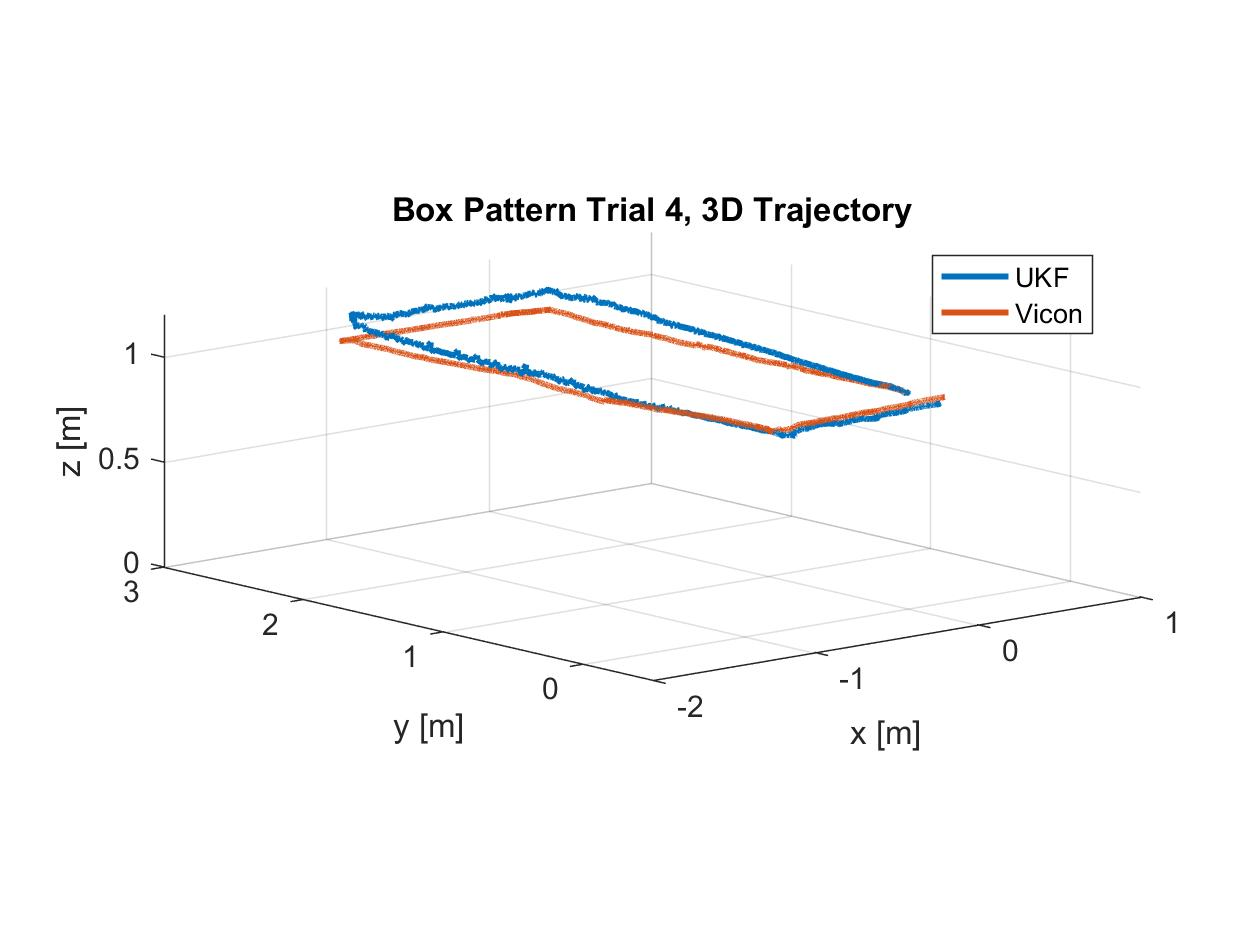
\includegraphics[width=\textwidth,right]{box4_3d}
    \end{subfigure}
    \caption[Box Pattern Trial 4 Trajectory]{2D and 3D trajectory plots from Box Pattern Trial~4.}
    \label{box4_traj}
\end{figure}

\begin{figure}
    \centering
    \begin{subfigure}{0.4\textwidth}
        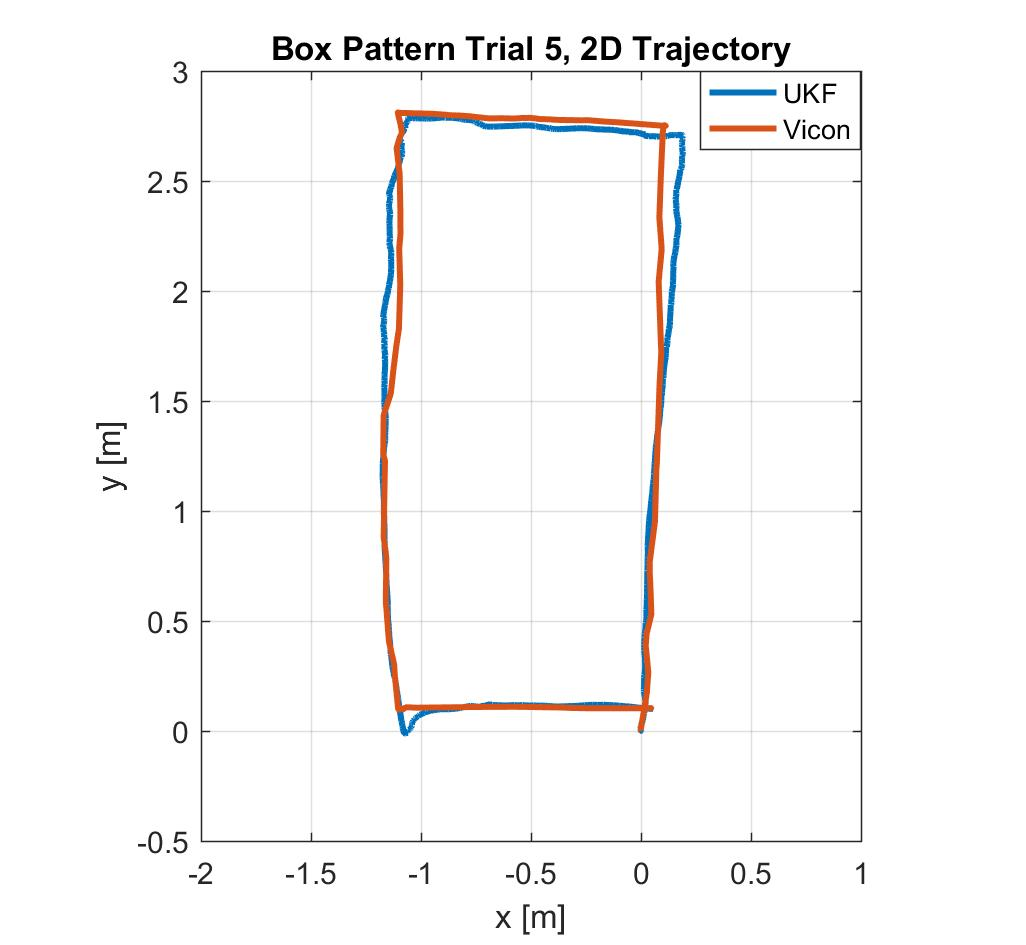
\includegraphics[width=\textwidth,left]{box5_2d}
    \end{subfigure}%
    ~ 
    \begin{subfigure}{0.6\textwidth}
        \centering
        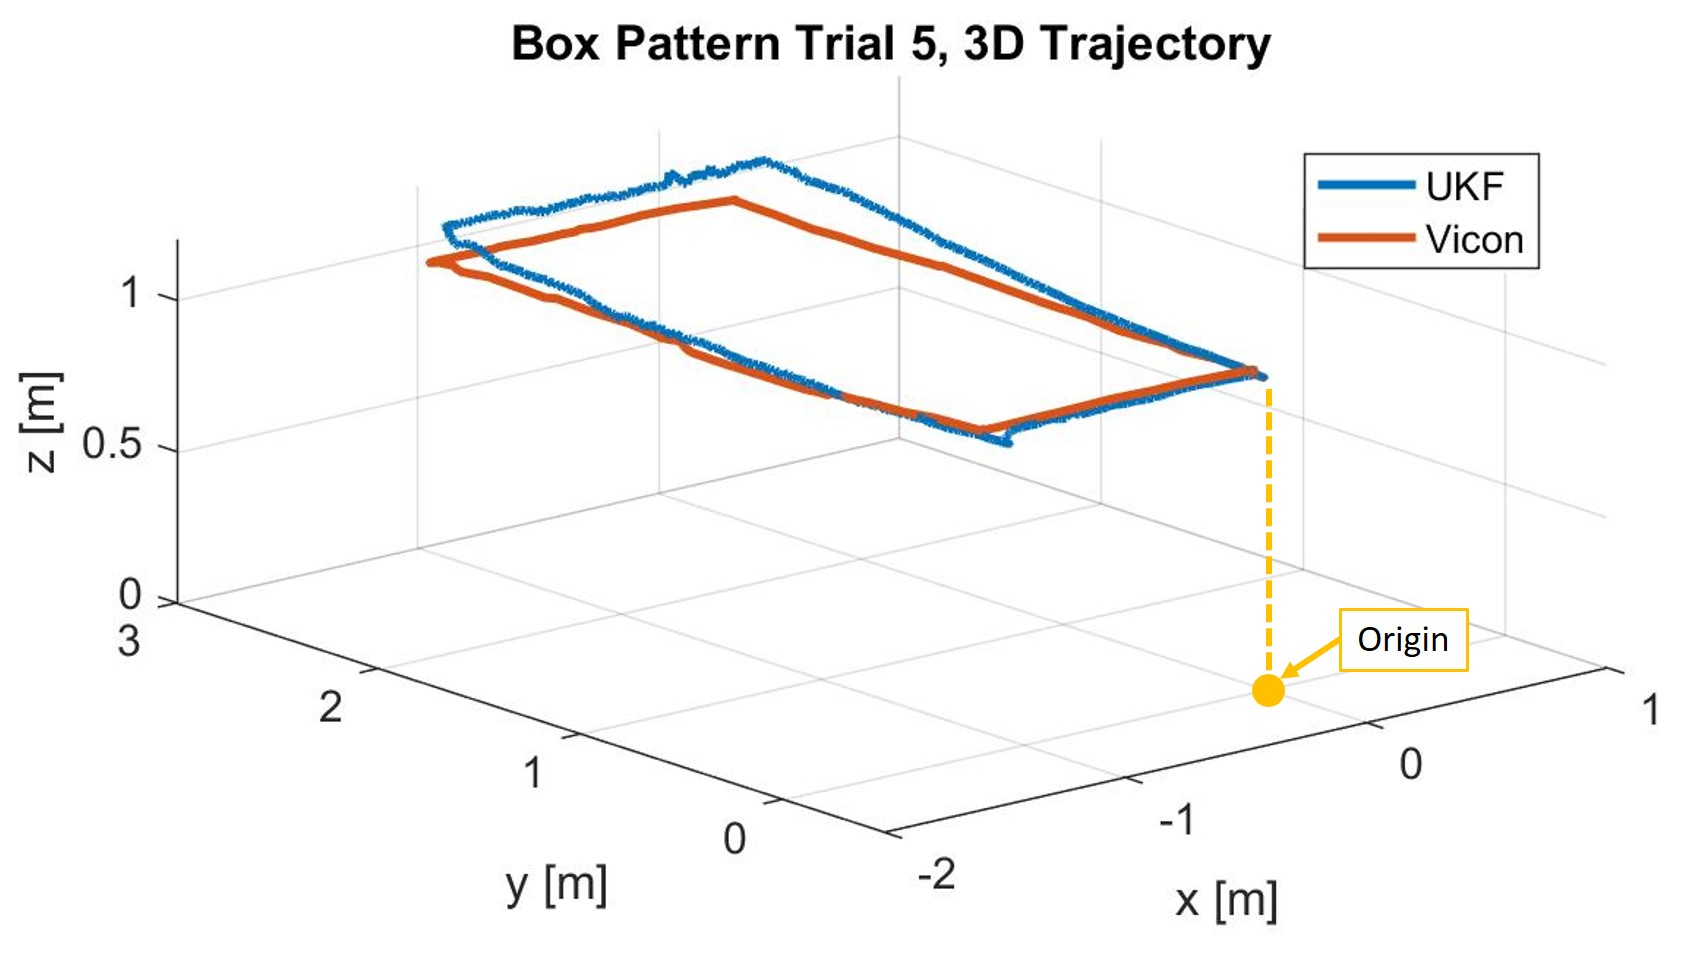
\includegraphics[width=\textwidth,right]{box5_3d}
    \end{subfigure}
    \caption[Box Pattern Trial 5 Trajectory]{2D and 3D trajectory plots from Box Pattern Trial~5.}
    \label{box5_traj}
\end{figure}